% Apresentação de 5 minutos da entrega parcial (MO438), com as redes direcionadas.
%
% apresentacao.tex gera os slides; roteiro.tex gera o roteiro de fala (as notas \note{} de cada
% slide, com a miniatura do slide). No Overleaf: Menu -> Main document -> roteiro.tex.
%
% As figuras em figuras/ são geradas e não se editam à mão:
%   graus.pdf, clusterizacao_local.pdf, cópias de report/entrega-parcial-direcionada/figuras/
%   distancias.pdf, componentes.pdf     (scripts/partial_delivery/export_networks.py --sym directed)
%   graus_pk.pdf,                       scripts/partial_delivery/draw_presentation.py
%   rede_<rede>_{tema,palavra}.pdf
% Os números vêm de entrega-parcial-direcionada/tabelas/metricas.tex, de tabelas/arcos.csv
% (draw_presentation.py) e de entrega-parcial-visualizacao/tabelas/blocos.tex.

\documentclass[aspectratio=169,11pt]{beamer}

\usetheme[progressbar=frametitle, numbering=fraction]{metropolis}
\usepackage[utf8]{inputenc}
\usepackage[T1]{fontenc}
\usepackage[brazil]{babel}
\usepackage{booktabs}
\usepackage{qrcode}
\usepackage{tikz}
\usetikzlibrary{arrows.meta, positioning, decorations.pathreplacing, fit, backgrounds}

\definecolor{mAzul}{HTML}{3B6EA8}

% ------------------------------------------------------------
% Roteiro: notas
% ------------------------------------------------------------
\ifdefined\comnotas
  \setbeameroption{show only notes}
\fi

\setbeamercolor{note page}{bg=white, fg=black}
\setbeamercolor{note title}{bg=white, fg=black}
\setbeamertemplate{note page}{%
  \vspace*{1mm}%
  \noindent
  \parbox[t]{0.76\linewidth}{%
    \vspace{0pt}\small\raggedright
    \setlength{\parskip}{4pt}%
    \insertnote}%
  \hfill
  \parbox[t]{0.21\linewidth}{\vspace{2mm}\insertslideintonotes{0.18}}%
}

\newcommand{\tempo}[1]{{\color{mLightBrown}\bfseries #1}\par}
\newcommand{\fala}{\textbf{Fala.} }
\newcommand{\aponte}{\textbf{Aponte:} }
\newcommand{\transicao}{\textbf{Transição:} }
\newcommand{\tema}{\scriptsize\color{mDarkTeal!65}}

% Um QR code (#2) num cartão, com o título (#3) e a descrição (#4) ao lado, a partir do
% ponto #1 (canto esquerdo, na altura do meio do cartão). Só dentro de um tikzpicture.
\newcommand{\cartaoqr}[4]{%
  \node[inner sep=0pt, anchor=west] (qr) at (#1) {\qrcode[height=1.4cm]{#2}};
  \node[anchor=west, align=left, font=\footnotesize, text width=3.9cm, right=3mm of qr] (rot)
    {\textbf{#3}\\[2pt]{\scriptsize\color{mDarkTeal!70}#4}};
  \begin{scope}[on background layer]
    \node[draw=mDarkTeal!25, fill=mDarkTeal!4, rounded corners=4pt, inner sep=5pt,
          fit=(qr) (rot)] {};
  \end{scope}}

% Uma rede desenhada à esquerda (#1, em figuras/) e o texto à direita (#2).
\newcommand{\rede}[2]{%
  \vspace*{9mm}% desce o desenho: a área do frame termina bem acima da borda do slide
  \begin{columns}[c]
  \begin{column}{0.70\textwidth}
    \centering\includegraphics[width=\linewidth, height=0.75\textheight,
                                keepaspectratio]{figuras/#1}
  \end{column}
  \begin{column}{0.29\textwidth}
    \footnotesize #2
  \end{column}
  \end{columns}}

% ------------------------------------------------------------
% Diagrama: uma rede pequena com 6 ocorrências de 3 tokens (mesma cor = mesmo token).
% As posições ficam fixas; só os arcos, passados como argumento, mudam.
% ------------------------------------------------------------
\tikzset{
  pics/minirede/.style={code={
    \coordinate (-a1) at (0.00, 0.65); \coordinate (-a2) at (0.45, 1.05);
    \coordinate (-b1) at (1.15, 1.00); \coordinate (-b2) at (1.50, 0.50);
    \coordinate (-c1) at (0.20, 0.05); \coordinate (-c2) at (1.00, 0.15);
    \foreach \u/\v in #1
      \draw[mDarkTeal!55, line width=0.7pt, -{Stealth[length=1.4mm]}, shorten >=1.3mm,
            shorten <=1.1mm] (-\u) -- (-\v);
    \foreach \n/\cor in {a1/mLightBrown, a2/mLightBrown, b1/mAzul, b2/mAzul,
                         c1/mLightGreen, c2/mLightGreen}
      \fill[\cor] (-\n) circle (1.15mm);
  }},
}

% ------------------------------------------------------------
% Diagrama: um vetor desenhado como uma fileira de casas, a partir do canto inferior esquerdo.
% Cada valor vai de -100 (laranja) a 100 (azul); 0 é branco. Os valores são ilustrativos.
% ------------------------------------------------------------
\tikzset{
  pics/vetor/.style={code={
    \edef\valores{#1}%
    \foreach \v [count=\i] in \valores {
      \ifnum\v<0 \colorlet{casa}{mLightBrown!\the\numexpr-\v\relax!white}%
      \else \colorlet{casa}{mAzul!\v!white}\fi
      \filldraw[fill=casa, draw=mDarkTeal!30, line width=0.3pt]
        ({(\i-1)*0.28}, 0) rectangle ++(0.28, 0.28);
    }
  }},
}

% ------------------------------------------------------------
\title{Da Rede Lexical à Rede Contextual}
\subtitle{Reorganização das representações internas de Transformers com Redes Complexas}
\author{Juliana Midlej do Espirito Santo \quad (RA 200208)}
\institute{MO438 -- Redes Complexas \quad·\quad Entrega parcial}
\date{}

\begin{document}

% ============================================================
\maketitle

\note{%
\textbf{Roteiro -- 5 minutos.} Alvo: \textbf{4min35s} (25 s de folga), cerca de 690 palavras
faladas (uns 150 por minuto), sem pressa. As marcas de tempo de cada página dizem onde você deve
estar. Os desenhos das redes são rápidos: 10 a 20 s cada.

\textbf{Três ideias que o público precisa levar:}
(1) cada camada do modelo vira uma rede sobre \emph{as mesmas} ocorrências de tokens;
(2) a rede deixa de ser organizada pela identidade do token, e no meio do modelo aparece o tema;
(3) no fim aparece outra organização: \emph{hubs} e a posição do token na palavra.

\textbf{Se o tempo apertar:} no slide dos graus, diga só a última frase; os de clusterização e
de componentes podem passar sem fala; no de L01, diga só ``no bloco 1, quase nada muda''; na
construção, pule ``no máximo 50 por token''. Marcas de controle: \textbf{2:05} ao sair da
construção, \textbf{3:05} ao sair das componentes, \textbf{4:20} ao sair do último desenho.

\tempo{0:00 → 0:10}
\fala Boa tarde! Eu sou a Juliana. O meu projeto usa redes complexas para ver como um modelo de
linguagem reorganiza as palavras, camada a camada.
}

% ============================================================
\begin{frame}{A mesma palavra, contextos diferentes}
\centering
% Uma palavra vira tokens (a divisão real do tokenizador do Qwen3), cada token ganha um vetor e
% cada bloco atualiza o vetor com os tokens anteriores (as linhas dentro dos blocos).
\begin{tikzpicture}[
    token/.style={draw=mDarkTeal!50, fill=mDarkTeal!8, rounded corners=2pt, font=\small,
                  inner sep=2pt, minimum width=9mm, minimum height=3.4mm},
    bloco/.style={draw=mDarkTeal, fill=mDarkTeal!8, rounded corners=2pt},
    seta/.style={-{Stealth[length=1.4mm]}, mDarkTeal!70},
    rotulo/.style={font=\scriptsize, align=center, text=mDarkTeal, anchor=south}]
  \def\linhas{1/0.6, 2/0.2, 3/-0.2, 4/-0.6}
  \node[font=\small\bfseries] (palavra) at (0.7,0) {polissêmica};
  \foreach \t/\i/\y in {pol/1/0.6, iss/2/0.2, êm/3/-0.2, ica/4/-0.6} {
    \node[token] (t\i) at (2.7,\y) {\t};
    \draw[mDarkTeal!50] (palavra.east) -- (t\i.west);
  }
  % os blocos: cada linha vai de um token para ele mesmo e para os seguintes
  \foreach \x/\nome in {5.6/bloco 1, 9.6/bloco 36} {
    \draw[bloco] (\x,-0.82) rectangle ++(1.0,1.64);
    \foreach \i/\yi in \linhas
      \foreach \j/\yj in \linhas {
        \ifnum\j<\i\relax\else
          \draw[mDarkTeal!45, line width=0.4pt] (\x+0.12,\yi) -- (\x+0.88,\yj);
        \fi}
    \node[rotulo, font=\footnotesize\bfseries] at (\x+0.5,0.88) {\nome};
  }
  \node at (8.96,0) {$\cdots$};
  % valores ilustrativos: o bloco 1 muda pouco o vetor; o bloco 36, muito
  \foreach \i/\y/\lex/\um/\fim in {
      1/0.6/{60,-30,10,-70}/{55,-20,15,-60}/{-60,40,70,-20},
      2/0.2/{-50,20,80,-10}/{-40,30,70,-20}/{20,-70,-30,60},
      3/-0.2/{30,70,-60,20}/{35,60,-50,30}/{-40,30,60,-70},
      4/-0.6/{-20,-80,40,60}/{-10,-70,50,50}/{70,10,-50,-30}} {
    \draw[seta] (t\i.east) -- (3.7,\y);
    \pic at (3.75,\y-0.14) {vetor=\lex};
    \draw[seta] (4.95,\y) -- (5.57,\y);
    \draw[seta] (6.63,\y) -- (7.15,\y);
    \pic at (7.2,\y-0.14) {vetor=\um};
    \draw[seta] (10.63,\y) -- (11.15,\y);
    \pic at (11.2,\y-0.14) {vetor=\fim};
  }
  \node[rotulo] at (0.7,0.88) {palavra};
  \node[rotulo] at (2.7,0.88) {tokens};
  \node[rotulo] at (4.31,0.88) {vetor inicial};
  \node[rotulo, anchor=north] at (4.31,-0.8) {2.560 números};
  \node[rotulo] at (11.76,0.88) {vetor final};
  \node[rotulo, anchor=north east] at (12.32,-0.9)
    {cada bloco atualiza o vetor com os \textbf{tokens anteriores}};

  % o modelo só vê as palavras anteriores, então o contexto de "banco" vem antes dele
  \begin{scope}[yshift=-2.65cm,
      frase/.style={draw=mDarkTeal!35, rounded corners=2pt, font=\small, inner sep=4pt,
                    align=left, text width=6.6cm, anchor=west},
      rotulo/.style={font=\footnotesize, align=center, text=mDarkTeal, anchor=south}]
  \node[frase] (a) at (0,0)
    {o cheque foi levado ao \alert{\textbf{banco}}\hspace{3mm}\hfill{\tema economia}};
  \node[frase] (b) at (0,-0.6)
    {a consulta SQL acessa o \alert{\textbf{banco}}\hspace{3mm}\hfill{\tema computação}};
  \node[frase] (c) at (0,-1.2)
    {a areia do rio formou um \alert{\textbf{banco}}\hspace{3mm}\hfill{\tema geografia}};
  \foreach \f/\y/\fim in {a/0/{80,30,-50,-20}, b/-0.6/{-70,60,10,-40},
                          c/-1.2/{-20,-40,70,50}} {
    \draw[mDarkTeal!50] (\f.east) -- (7.45,\y);
    \pic at (7.5,\y-0.14) {vetor={40,-60,20,70}};
    \draw[seta] (8.7,\y) -- (10.35,\y);
    \pic at (10.4,\y-0.14) {vetor=\fim};
  }
  \node[rotulo] at (8.06,0.24) {\textbf{mesmo token}\\na entrada};
  \node[rotulo] at (10.96,0.24)
    {\alert{\textbf{representações diferentes}}\\conforme o contexto};
  \end{scope}
\end{tikzpicture}

\begin{alertblock}{Pergunta}
Como as relações de semelhança entre os tokens mudam ao longo das camadas?
\end{alertblock}
\end{frame}

\note{%
\tempo{0:10 → 0:40}
\fala O modelo divide o texto em tokens: palavras ou partes de palavras; ``polissêmica'', por
exemplo, vira quatro tokens. Cada token começa com um vetor, uma lista de números. A cada
camada, sua representação é atualizada com informações do texto anterior. Aqui, o mesmo token
``banco'' aparece em três contextos. Sabemos que o contexto muda essas representações. Neste
trabalho, queremos entender como isso reorganiza as relações de semelhança entre elas.

\aponte o esquema de cima, da esquerda para a direita; depois, as frases com ``banco''.

\textbf{Se perguntarem:} a divisão de ``polissêmica'' é a do Qwen3; as cores são ilustrativas
(cada casa é um número). O modelo só olha para o texto anterior (as linhas nos blocos); por
isso, nos exemplos, o contexto vem antes de ``banco''. O vetor inicial (\emph{embedding}) é o
mesmo quando o token é o mesmo.

\transicao ``Para responder, eu transformo cada camada numa rede.''
}

% ============================================================
\begin{frame}{A ideia: uma rede por camada, sempre com os mesmos vértices}
\centering
\begin{tikzpicture}[
    bloco/.style={draw=mDarkTeal, fill=mDarkTeal!8, rounded corners=2pt, font=\small,
                  minimum height=7mm, inner xsep=5pt},
    seta/.style={-{Stealth[length=1.8mm]}, thick, mDarkTeal!70},
    tap/.style={-{Stealth[length=1.8mm]}, densely dashed, mLightBrown},
    rotulo/.style={font=\small, align=center}]
  \node[font=\small, align=center] (txt) at (0,0) {parágrafo\\da Wikipédia};
  \node[bloco] (emb) at (2.6,0) {\emph{embedding}};
  \node[bloco] (b1)  at (5.0,0) {bloco 1};
  \node (d1)         at (6.55,0) {$\cdots$};
  \node[bloco] (b18) at (8.1,0) {bloco 18};
  \node (d2)         at (9.65,0) {$\cdots$};
  \node[bloco] (b36) at (11.2,0) {bloco 36};
  \draw[seta] (txt) -- (emb);
  \draw[seta] (emb) -- (b1);
  \draw[seta] (b1) -- (d1);
  \draw[seta] (d1) -- (b18);
  \draw[seta] (b18) -- (d2);
  \draw[seta] (d2) -- (b36);
  \draw[decorate, decoration={brace, amplitude=4pt}, mDarkTeal!70]
    ([yshift=2mm]emb.north west) -- ([yshift=2mm]b36.north east)
    node[midway, above=4pt, font=\small] {Qwen3-4B-Base (36 blocos)};

  \foreach \no/\x/\nome/\arcos in {
      emb/2.6/lex/{a1/a2, a2/a1, b1/b2, b2/b1, c1/c2, c2/c1, c1/a1},
      b1/5.0/L01/{a1/a2, a2/a1, b1/b2, b2/b1, c1/c2, c2/c1, a2/b1},
      b18/8.1/L18/{a1/a2, a1/c1, b1/b2, a2/b1, b2/c2, c1/c2},
      b36/11.2/L36/{a1/c1, c1/a1, a2/b1, b2/b1, c2/b1, c1/c2}} {
    \draw[tap] (\no.south) -- (\x,-1.05);
    \pic at (\x-0.75,-2.35) {minirede=\arcos};
    \node[rotulo] at (\x,-2.75) {\textbf{\nome}};
  }
  \node[font=\scriptsize, text=mDarkTeal!70, anchor=west] at (-0.9,-1.8)
    {esquema:};
  \node[font=\scriptsize, text=mDarkTeal!70, anchor=west, align=left] at (-0.9,-2.25)
    {mesma cor =\\mesmo token};
\end{tikzpicture}

\vspace{2mm}
\begin{columns}[T]
\begin{column}{0.44\textwidth}
\textbf{Vértice:} uma \alert{ocorrência} de token\\
(as mesmas nas quatro redes)
\end{column}
\begin{column}{0.48\textwidth}
\textbf{Arco:} cada ocorrência aponta para as $k$ mais parecidas com ela
\end{column}
\end{columns}

\vspace{2mm}
Só o vetor muda $\Rightarrow$ as redes se comparam \alert{vértice a vértice}.
\end{frame}

\note{%
\tempo{0:40 → 1:05}
\fala A ideia é transformar cada camada numa rede. Eu guardo o vetor de cada ocorrência de token
em quatro pontos: na entrada e na saída dos blocos 1, 18 e 36, o último. Em cada ponto, cada
ocorrência aponta para as mais parecidas com ela. Os vértices são os mesmos nas quatro redes; só
muda o vetor. Então dá para comparar as redes vértice a vértice.

\aponte as duas bolinhas laranja (o mesmo token): ligadas na entrada, separadas no fim. É só
um esquema.

\transicao ``Com isso, o que eu quero descobrir é\ldots''
}

% ============================================================
\begin{frame}{Objetivos e hipóteses}
\textbf{Objetivo:} caracterizar, com redes complexas, \alert{quanto} e \alert{como} a estrutura
de semelhança muda entre a entrada e as camadas do modelo.

\vspace{2mm}
\small
\begin{columns}[T]
\begin{column}{0.52\textwidth}
\textbf{Perguntas}
\begin{description}[P1]
  \item[P1] Quanto a rede muda, local e globalmente?
  \item[P2] Em que camadas a mudança se concentra?
  \item[P3] Surgem comunidades de contexto (tema)?
  \item[P4] Um mesmo token se separa conforme o contexto (\emph{banco}, \emph{nota})?
\end{description}
\end{column}
\begin{column}{0.44\textwidth}
\textbf{Espera-se ver nas redes:}
\begin{itemize}
  \item menos arcos entre ocorrências do mesmo token
  \item clusterização menor
  \item mais arcos dentro do mesmo tema
\end{itemize}
\end{column}
\end{columns}
\end{frame}

\note{%
\tempo{1:05 → 1:30}
\fala O objetivo é medir quanto e como essa estrutura muda: quanto a rede muda, em que camadas,
se aparecem comunidades de contexto, como o tema, e se as ocorrências de ``banco'' se separam
pelo sentido. Eu espero menos arcos entre ocorrências do mesmo token, clusterização menor e
mais arcos dentro do mesmo tema.

\transicao ``Agora, como as redes foram construídas.''
}

% ============================================================
\begin{frame}{Como as redes foram construídas}
\small
\begin{columns}[T]
\begin{column}{0.32\textwidth}
\begin{block}{Vértices}
\begin{itemize}
  \item Wikipédia em português, \textbf{8 temas}, de física a futebol
  \item \alert{\textbf{13.606 ocorrências}} de 2.864 tokens (no máximo 50 por token)
  \item 74\%: todos os tokens de 80 parágrafos; o resto, palavras escolhidas
        (ex.: polissêmicas)
\end{itemize}
\end{block}
\end{column}
\begin{column}{0.32\textwidth}
\begin{block}{Vetores}
\begin{itemize}
  \item \textbf{Qwen3-4B-Base}: aberto, 36 blocos, dimensão 2.560
  \item cada parágrafo passa sozinho pelo modelo
  \item \textbf{lex}: o \emph{embedding} do token (igual em todas as ocorrências)
  \item \textbf{L01, L18, L36}: a saída dos blocos 1, 18 e 36
\end{itemize}
\end{block}
\end{column}
\begin{column}{0.32\textwidth}
\begin{block}{Arcos}
\begin{itemize}
  \item $i\to j$: $i$ aponta para as \alert{\textbf{$k=10$}} de maior \textbf{cosseno}, de
        qualquer parágrafo
  \item rede \textbf{direcionada}: grau de saída 10; o de \textbf{entrada} varia
  \item 136.060 arcos por rede
\end{itemize}
\end{block}
\end{column}
\end{columns}
\end{frame}

\note{%
\tempo{1:30 → 2:05}
\fala Os dados são artigos da Wikipédia em português, de oito temas. Os vértices são 13.606
ocorrências de cerca de 2.900 tokens, no máximo 50 por token. O modelo é o Qwen3, com 4 bilhões de
parâmetros e 36 blocos; na rede lex, o vetor é o \emph{embedding}, igual para todas as ocorrências
do token. Cada ocorrência aponta para as 10 mais parecidas pelo cosseno, em qualquer parágrafo.
Então a rede é direcionada: todo vértice tem grau de saída 10, e o grau de entrada, quantos o
escolheram, varia.

\transicao ``E o que as métricas mostram?''
}

% ============================================================
\begin{frame}{Resultados: grau, reciprocidade e clusterização}
\centering
{\small 13.606 vértices\enspace·\enspace 136.060 arcos\enspace·\enspace grau médio (entrada e
saída) 10\enspace·\enspace densidade $7{,}35\times 10^{-4}$}

\vspace{2mm}
\begin{tabular}{lcccc}
\toprule
 & \textbf{lex} & \textbf{L01} & \textbf{L18} & \textbf{L36} \\
\midrule
Grau de entrada máximo & 29 & 60 & 55 & 247 \\
Vértices com grau de entrada 0 & 0,7\% & 3,6\% & 0,7\% & 5,4\% \\
Reciprocidade (arcos com arco inverso) & 49,1\% & 57,3\% & 60,7\% & 43,7\% \\
Transitividade dirigida $T^{\rightarrow}$ & 0,440 & 0,510 & 0,325 & 0,230 \\
Clusterização local média $\bar C^{\rightarrow}$ & 0,437 & 0,534 & 0,331 & 0,296 \\
\midrule
Arcos entre ocorrências do mesmo token & 70,1\% & 69,4\% & 42,6\% & 25,1\% \\
Jaccard dos arcos com a rede anterior & --- & 0,316 & 0,181 & 0,162 \\
\bottomrule
\end{tabular}

\vspace{2mm}
{\scriptsize Todo vértice aponta para $k=10$: o grau de saída e a densidade são fixos; o que
varia é o grau de entrada.}
\end{frame}

\note{%
\tempo{2:05 → 2:25}
\fala Estas são as métricas das redes direcionadas. Na entrada, 70\% dos arcos ligam ocorrências do mesmo token; na última
camada, só 25\%. A transitividade e a clusterização caem quase pela metade. E, depois do bloco 1,
a sobreposição dos arcos com a rede anterior fica abaixo de 0,2.

\aponte a linha dos arcos do mesmo token e, depois, a do Jaccard.

\textbf{Se perguntarem:} a reciprocidade sobe até L18 (61\%) e cai em L36 (44\%), a camada em que
aparecem os \emph{hubs}.

\transicao ``E quem alcança quem?''
}

% ============================================================
\begin{frame}{Resultados: componentes e distâncias}
\centering
\footnotesize
\setlength{\tabcolsep}{3pt}
\renewcommand{\arraystretch}{0.92}
\begin{tabular}{lcccc}
\toprule
 & \textbf{lex} & \textbf{L01} & \textbf{L18} & \textbf{L36} \\
\midrule
Componentes fracas & 44 & 40 & 2 & 2 \\
Componentes fortes & 1.059 & 1.768 & 173 & 1.517 \\
Maior componente forte (vértices) & 2.640 (19\%) & 3.862 (28\%) & 12.997 (96\%) & 10.930 (80\%) \\
Pares ordenados com caminho & 17,7\% & 25,4\% & 95,1\% & 80,2\% \\
\midrule
(a) Distância média (pares com caminho) & 10,37 & 11,28 & 6,97 & 9,96 \\
(a) Maior distância finita & 33 & 39 & 20 & 50 \\
(b) Distância média na maior comp.\ forte & 9,80 & 10,36 & 6,95 & 9,73 \\
(b) Diâmetro da maior comp.\ forte & 30 & 37 & 20 & 50 \\
(c) Eficiência global $E$ & 0,020 & 0,027 & 0,147 & 0,100 \\
(c) Distância harmônica $1/E$ & 49,41 & 36,86 & 6,79 & 9,98 \\
\bottomrule
\end{tabular}

\vspace{1mm}
{\scriptsize Componente forte: todos se alcançam seguindo os arcos (fraca: sem o sentido).
Sem caminho, $d=\infty$:\\ (a) só pares com caminho; (b) só a maior comp.\ forte; (c) $E$ é a
média de $1/d$, com $1/\infty=0$.\par}

{\small lex $\approx$ L01: grupos fechados por token $\;\longrightarrow\;$
L18: quase todos se alcançam $\;\longrightarrow\;$ L36: \emph{hubs}}
\end{frame}

\note{%
\tempo{2:25 → 2:45}
\fala As componentes fortes, onde todo mundo alcança todo mundo, contam a mesma história: em lex,
os grupos de um token apontam só para dentro, e só 18\% dos pares têm caminho. Em L18, a maior
componente forte tem 95\% dos vértices, e as distâncias são as menores. Em L36, o alcance cai
para 80\%.

\aponte a linha dos pares com caminho e, depois, a da eficiência.

\transicao ``As figuras mostram as distribuições.''
}

% ============================================================
\begin{frame}{Resultados: distribuição dos graus de entrada}
\centering
\vspace*{7mm}
\begin{columns}[T]
\begin{column}{0.49\textwidth}
\centering
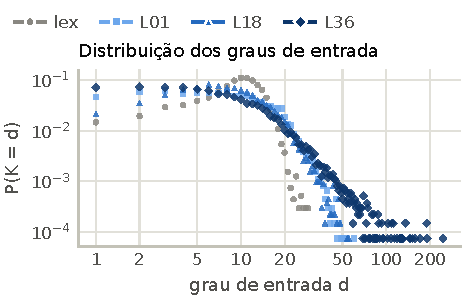
\includegraphics[width=\linewidth]{figuras/graus_pk.pdf}
\end{column}
\begin{column}{0.49\textwidth}
\centering
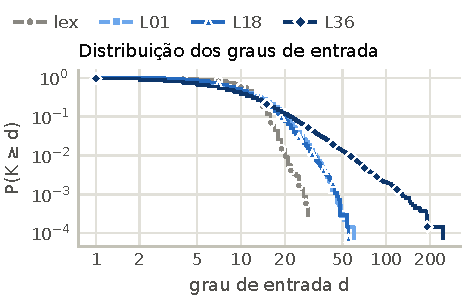
\includegraphics[width=\linewidth]{figuras/graus.pdf}
\end{column}
\end{columns}
\end{frame}

\note{%
\tempo{2:45 → 2:55}
\fala O grau de entrada: à esquerda, a fração de vértices com cada grau; à direita, com pelo
menos esse grau. Em L36 a cauda vai até 247: são os \emph{hubs}.

\textbf{Se perguntarem:} $P(K=d)$ é a fração de vértices com grau de entrada exatamente $d$, e
$P(K\ge d)$, com pelo menos $d$. O piso perto de $10^{-4}$ é um vértice só (1 em 13.606). Os de
grau 0 (0,7\% a 5,4\%) não cabem no eixo logarítmico.

\textbf{Se o tempo apertar:} diga só a última frase.
}

% ============================================================
\begin{frame}{Resultados: clusterização local e distâncias}
\centering
\vspace*{7mm}
\begin{columns}[T]
\begin{column}{0.49\textwidth}
\centering
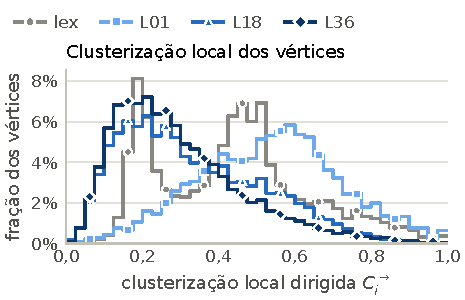
\includegraphics[width=\linewidth]{figuras/clusterizacao_local.pdf}
\end{column}
\begin{column}{0.49\textwidth}
\centering
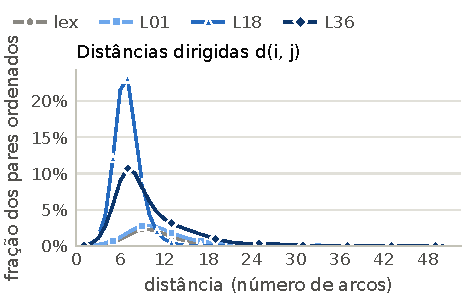
\includegraphics[width=\linewidth]{figuras/distancias.pdf}
\end{column}
\end{columns}
\end{frame}

\note{%
\tempo{2:55 → 3:00}
\fala A clusterização local cai para perto de 0,2, e em L18 os pares ficam mais perto.

\textbf{Se perguntarem:} a área sob cada curva das distâncias é a fração de pares com caminho; os
demais têm distância infinita.
}

% ============================================================
\begin{frame}{Resultados: componentes fortes}
\centering
\vspace*{10mm}
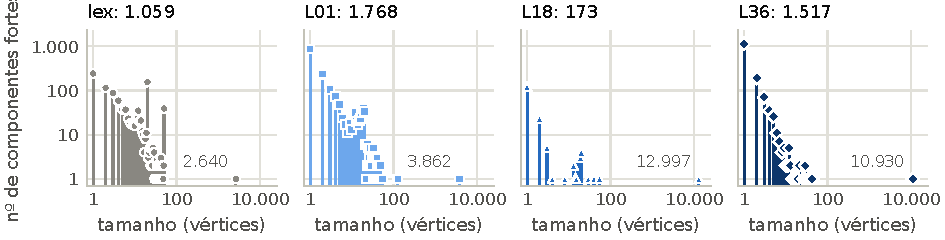
\includegraphics[width=\linewidth]{figuras/componentes.pdf}
\end{frame}

\note{%
\tempo{3:00 → 3:05}
\fala E as componentes fortes: em L18, uma só reúne quase toda a rede.

\textbf{Se perguntarem:} cada painel dá quantas componentes fortes (eixo vertical) têm cada
tamanho (eixo horizontal); o título dá o total, e o rótulo, o tamanho da maior.

\transicao ``E como essas redes ficam desenhadas?''
}

% ============================================================
\begin{frame}{Visualização: lex, o \emph{embedding} de entrada}
\rede{rede_lex_tema.pdf}{%
\begin{itemize}
  \item Centenas de \textbf{grupos pequenos}.
  \item Temas misturados: só \alert{22\%} dos arcos ligam ocorrências do mesmo tema.
\end{itemize}}
\end{frame}

\note{%
\tempo{3:05 → 3:20}
\fala Agora os desenhos, um por rede. O layout é UMAP, as cores são os temas, e o desenho ignora
o sentido dos arcos. Na entrada, a rede é um monte de grupinhos, quase sempre ocorrências de um
mesmo token, com os temas misturados.
}

% ============================================================
\begin{frame}{Visualização: L01, saída do bloco 1}
\rede{rede_L01_tema.pdf}{%
\begin{itemize}
  \item Quase igual a lex: grupos de um token, temas misturados.
  \item 69\% dos arcos no mesmo token; 24\% no mesmo tema.
\end{itemize}}
\end{frame}

\note{%
\tempo{3:20 → 3:30}
\fala No bloco 1, quase nada muda: ainda grupinhos de um token, com temas misturados, como a
tabela já mostrava.
}

% ============================================================
\begin{frame}{Visualização: L18, saída do bloco 18}
\rede{rede_L18_tema.pdf}{%
\begin{itemize}
  \item Os grupos se fundem num \textbf{bloco central}.
  \item Surgem \alert{regiões de um tema}: física (azul), computação (rosa)\ldots
  \item \alert{55\%} dos arcos no mesmo tema; assortatividade por tema de 0,10 (lex) para
        \alert{0,48}.
\end{itemize}}
\end{frame}

\note{%
\tempo{3:30 → 3:50}
\fala No bloco 18, os grupos se fundem num bloco central, e aparecem regiões de um tema só, como
física em azul e computação em rosa. Mais da metade dos arcos, 55\%, liga ocorrências do mesmo
tema. O contexto aparece no meio do modelo.

\aponte a região azul e a rosa.
}

% ============================================================
\begin{frame}{Visualização: L36, saída do bloco 36}
\rede{rede_L36_tema.pdf}{%
\begin{itemize}
  \item A rede se divide em \textbf{dois blocos}.
  \item O tema perde força: \alert{47\%} dos arcos no mesmo tema (55\% em L18).
  \item O que separa os blocos?
\end{itemize}}
\end{frame}

\note{%
\tempo{3:50 → 4:00}
\fala No último bloco, a rede se divide em dois blocos, e o tema perde força: 47\% dos arcos. O
que separa os dois blocos?
}

% ============================================================
\begin{frame}{Visualização: L36, cor pela posição do token na palavra}
\rede{rede_L36_palavra.pdf}{%
\begin{itemize}
  \item {\color{mAzul}\textbf{Azul}}: a palavra \textbf{continua} no token seguinte (pedaço do
        começo ou do meio de uma palavra); 29\% dos vértices.
  \item O bloco menor é \alert{94\% azul}.
  \item Arcos entre azul e cinza: 14\% em lex, \alert{2\%} em L36; assortatividade
        \alert{0,94}.
\end{itemize}}
\end{frame}

\note{%
\tempo{4:00 → 4:20}
\fala É a posição do token na palavra. Em azul, os tokens em que a palavra continua no token
seguinte, como os pedaços de uma palavra longa. O bloco menor é 94\% azul. Perto da saída, o
modelo agrupa os tokens pelo que vem depois, e não pelo tema. Essa foi a surpresa da
visualização.

\aponte o bloco azul.

\textbf{Se perguntarem:} isso combina com a tarefa do modelo, que é prever o próximo token; é uma
interpretação, ainda não testada.
}

% ============================================================
\begin{frame}{Síntese}
\begin{columns}
\begin{column}{0.78\textwidth}
\textbf{O que a entrega parcial mostra}
\begin{itemize}
  \item A rede deixa de ser organizada pelo token: arcos do mesmo token de
        \alert{70\% → 25\%}.
  \item No meio (L18), quase todos se alcançam e aparece o \alert{tema}.
  \item No fim (L36), aparecem \emph{hubs} e a divisão pela \alert{posição na palavra}.
\end{itemize}
\end{column}
\end{columns}

\vspace{7mm}
\centering
\begin{tikzpicture}
  \cartaoqr{0,0}{https://annwith.github.io/gender-representation-networks/redes/}
    {Redes interativas}{as quatro redes, no navegador}
  \cartaoqr{6.7,0}{https://github.com/annwith/gender-representation-networks}
    {Repositório e dados}{código e arquivos GraphML}
\end{tikzpicture}
\end{frame}

\note{%
\tempo{4:20 → 4:35}
\fala Resumindo: a rede deixa de ser organizada pelo token; no meio aparece o tema; e no fim,
\emph{hubs} e a divisão pela posição na palavra. As redes interativas estão no QR code.
Obrigada!
}

% ------------------------------------------------------------
% Perguntas prováveis (só no roteiro)
% ------------------------------------------------------------
\note{%
\textbf{Perguntas prováveis (1/3)}

\textbf{Por que $k$ vizinhos e não um limiar de similaridade?} Com $k$ fixo, toda ocorrência faz
o mesmo número de escolhas em todas as camadas. A distribuição dos cossenos muda de uma camada
para outra, então o mesmo limiar daria redes de densidades muito diferentes.

\textbf{Por que a rede direcionada?} É o que o $k$-NN produz: $i$ escolher $j$ não implica o
contrário (só 44\% a 61\% dos arcos têm o arco inverso). Como o grau de saída é fixo em 10, a
informação está no grau de entrada, que mostra os \emph{hubs}. A versão não direcionada (por
união) também foi calculada e mostra a mesma tendência.

\textbf{E a distância média?} Muitos pares não têm caminho (82\% em lex), e a distância deles é
infinita. Entre os pares com caminho, a média é 10,4 (lex), 11,3 (L01), 7,0 (L18) e 10,0 (L36):
L18 é a rede em que se chega mais longe e mais rápido.
}

\note{%
\textbf{Perguntas prováveis (2/3)}

\textbf{E os empates na rede lex?} Ocorrências do mesmo token têm o mesmo vetor (cosseno 1), então
quem entra entre os 10 vizinhos é sorteado, com semente fixa. Por isso o Jaccard entre lex e L01
(0,32) subestima a semelhança. A robustez a outras sementes e a outros tratamentos de empate
ainda não foi testada.

\textbf{Por que o Qwen3-4B-Base?} É aberto, atual, multilíngue, tem 36 blocos (dá para fazer a
curva camada a camada) e cabe numa GPU de 8 GiB. A versão \emph{Base} é o modelo treinado só para
prever o próximo token, sem o ajuste para conversa. O custo é que ele quebra muito o português em
pedaços; por isso as medidas são separadas por categoria de token.

\textbf{Por que só quatro camadas?} A entrega parcial compara entrada, início, meio e fim. Os
vetores das 36 camadas já foram extraídos, para a curva camada a camada.
}

\note{%
\textbf{Perguntas prováveis (3/3)}

\textbf{O que é o tema?} A categoria da Wikipédia de onde veio o artigo (``esporte'' é a
categoria Futebol).

\textbf{Por que o desenho não tem setas?} Com 136 mil arcos, as setas não seriam legíveis. O UMAP
usa os arcos sem o sentido; ele aproxima vértices ligados e afasta os não ligados. A posição e a
orientação absolutas não têm significado. Cada slide mostra o miolo da rede; de 2\% a 4\% dos
vértices ficam de fora (eles estão na página interativa).

\textbf{\emph{Hubs}?} Em espaços de alta dimensão, algumas representações viram vizinhas de muitas
outras (\emph{hubness}). Em L36, uma ocorrência é escolhida por 247 outras, e 5,4\% não são
escolhidas por ninguém.

\textbf{De onde vêm os 94\%?} Das comunidades (Leiden, resolução baixa) da visualização: o
bloco menor de L36 tem 4.012 vértices, e 94\% deles são ``continua''.
}

\end{document}
